%!TEX root = slides.tex

\section{Algorithms}

\begin{frame}{Decision tree}
  \begin{description}
    \item[Decision trees] are rooted trees where each vertex represents a decision.
    \vspace{2mm}
    \item[Possible results] of each decision are represented by the edges.
    \vspace{2mm}
    \item[These edges] connect the decision vertex to the vertices representing the outcomes, at the next level down.
    \vspace{2mm}
    \item[These vertices] is turn can represent more decisions.
    \vspace{2mm}
    \item[Final outcomes] of the procedure are represented by the leaves.
  \end{description}
\end{frame}

\begin{frame}[fragile]{Decision tree example}

  \begin{center}
    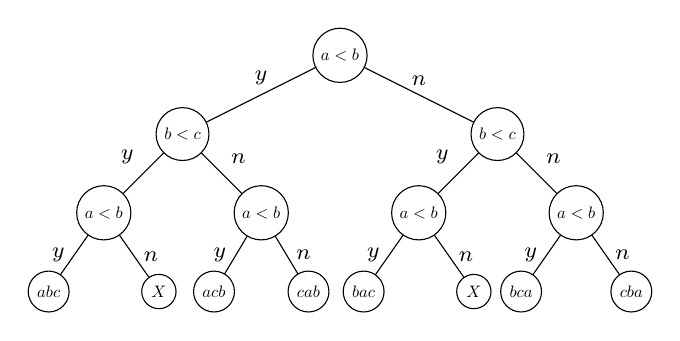
\begin{tikzpicture}
    \begin{scope}[every node/.style={circle,draw,scale=0.6}]
    \node (a) at (3,4) {$a<b$};
    \node (b) at (1,3) {$b<c$};
    \node (c) at (5,3) {$b<c$};
    \node (d) at (0,2) {$a<b$};
    \node (e) at (2,2) {$a<b$};
    \node (f) at (4,2) {$a<b$};
    \node (g) at (6,2) {$a<b$};
    \node (h) at (-0.7,1) {$abc$};
    \node (i) at (0.7,1) {$X$};
    \node (j) at (1.4,1) {$acb$};
    \node (k) at (2.6,1) {$cab$};
    \node (l) at (3.3,1) {$bac$};
    \node (m) at (4.7,1) {$X$};
    \node (n) at (5.3,1) {$bca$};
    \node (o) at (6.7,1) {$cba$};
    \end{scope}
    \begin{scope}[every edge/.style={draw=black}]
    \path (a) edge node[above] {\footnotesize $y$} (b);
    \path (a) edge node[above] {\footnotesize $n$} (c);
    \path (b) edge node[above left] {\footnotesize $y$} (d);
    \path (b) edge node[above right]  {\footnotesize $n$} (e);
    \path (c) edge node[above left] {\footnotesize $y$} (f);
    \path (c) edge node[above right]  {\footnotesize $n$} (g);
    \path (d) edge node[left] {\footnotesize $y$} (h);
    \path (d) edge node[right]  {\footnotesize $n$} (i);
    \path (e) edge node[left] {\footnotesize $y$} (j);
    \path (e) edge node[right]  {\footnotesize $n$} (k);
    \path (f) edge node[left] {\footnotesize $y$} (l);
    \path (f) edge node[right]  {\footnotesize $n$} (m);
    \path (g) edge node[left] {\footnotesize $y$} (n);
    \path (g) edge node[right]  {\footnotesize $n$} (o);
    \end{scope}
    \end{tikzpicture}
  \end{center}
\end{frame}

\begin{frame}{Height of a decision tree}
  \begin{description}
    \item[The height] of a decision tree is the maximum distance from root to leaf (as usual).
    \vspace{2mm}
    \item[Each] internal vertex represents a decision.
    \vspace{2mm}
    \item[The height] therefore is the maximium number of decisions made when starting from the root of the tree.
  \end{description}
\end{frame}
